% ------------------------------------------------------------------------------
% ------------------------------------------------------------------------------
% Relatório do Exercício 3 de Algoritmos Numéricos 2
% Autor: André Barreto Silveira
% ------------------------------------------------------------------------------
% ------------------------------------------------------------------------------

\documentclass[
	11pt,				% tamanho da fonte
	oneside,			% para impressão apenas no verso. Oposto a twoside
	a4paper,			% tamanho do papel. 
	english,			% idioma adicional para hifenização
	brazil,				% o último idioma é o principal do documento
	]{article}


% ---
% PACOTES
% ---
\usepackage{lmodern}
\usepackage[T1]{fontenc}
\usepackage[utf8]{inputenc}
\usepackage{indentfirst}
\usepackage{nomencl}
\usepackage{color}
\usepackage{graphicx}
\usepackage{microtype}
\usepackage{makeidx}
\usepackage{multirow,tabularx}
\usepackage{multicol}
\usepackage{listings}
\usepackage{color}
\usepackage{hyperref}
\usepackage{cite}
\usepackage{url}
\usepackage[brazilian]{babel}
\usepackage[brazilian,hyperpageref]{backref}
\usepackage[fleqn]{amsmath}
\usepackage{mathtools,amssymb}
\usepackage{pgfplots}

\usepackage{lipsum}
% ---

% ---
% Configurações do pacote listings
% ---
\definecolor{mygreen}{rgb}{0,0.6,0}
\definecolor{mygray}{rgb}{0.571428571,0.571428571,0.571428571}
\definecolor{mymauve}{rgb}{0.5714285718,0,0.82}
\definecolor{codegreen}{rgb}{0,0.6,0}
\definecolor{codegray}{rgb}{0.571428571,0.571428571,0.571428571}
\definecolor{codepurple}{rgb}{0.5714285718,0,0.82}
\definecolor{backcolour}{rgb}{0.95,0.95,0.92}
\lstset{
	backgroundcolor=\color{white},
	basicstyle=\footnotesize,
	breakatwhitespace=false,
	breaklines=true,
	captionpos=b,
	commentstyle=\color{mygreen},
	deletekeywords={...},
	escapeinside={\%*}{*)},
	extendedchars=true,
	keepspaces=true,
	keywordstyle=\color{blue},
	language=C,
	otherkeywords={*,...},
	numbers=left,
	numbersep=5pt,
	numberstyle=\tiny\color{mygray},
	rulecolor=\color{black},
	showspaces=false,
	showstringspaces=false,
	showtabs=false,
	stepnumber=1,
	stringstyle=\color{mymauve},
	tabsize=2,
	title=\lstname
}
% ---
	
% ---
% Informações de dados para CAPA
% ---
\title{\textbf{Solução de Problemas de Valor no Contorno Bidimensionais}}
\author{
André Barreto e Igor Ventorim\\\\
\normalsize Universidade Federal do Espírito Santo\\
}
\date{2015}
% ---

% ---
% Configurações de aparência do PDF final
% ---
\definecolor{blue}{RGB}{41,5,195}

% informações do PDF
\makeatletter
\hypersetup{
	pdftitle={\@title}, 
	pdfauthor={\@author},
	pdfsubject={Escalonamento de Jobs},
	pdfcreator={LaTeX with abnTeX2},
	pdfkeywords={abnt}{latex}{abntex}{abntex2}{atigo científico}, 
	colorlinks=true,
	linkcolor=blue,
	citecolor=blue,
	filecolor=magenta,
	urlcolor=blue,
	bookmarksdepth=4
}
\makeatother
% --- 

% ---
% Compila o indice
% ---
\makeindex
% ---

% --- 
% Espaçamentos entre linhas e parágrafos 
% --- 
\setlength{\parindent}{1cm}
\setlength{\parskip}{0.2cm}
% ---

% ----
% Início do documento
% ----
\begin{document}
% ---

% Seleciona o idioma do documento
\selectlanguage{brazil}

% Retira espaço extra obsoleto entre as frases.
\frenchspacing

\graphicspath{ {Imagens/} }

% ------------------------------------------------------------------------------
% Página de Título
% ------------------------------------------------------------------------------
\begin{titlepage}
	\centering
	{\scshape \large Universidade Federal do Espírito Santo\par}
	{\large Departamento de Informática\par}
	\vspace{1cm}
	{\large André Barreto Silveira\par}
	
	\vfill
	
	{\LARGE \bfseries Equação do Calor Unidimensional Transiente\par}
	\vspace{1cm}
	{\large Exercício 3 de Algoritmos Numéricos 2\par}

	\vfill

	{\large Vitória\par}
	{\large 2016\par}
\end{titlepage}
\addtocounter{page}{1}

% ------------------------------------------------------------------------------
% Introdução
% ------------------------------------------------------------------------------
\section{Introdução}
Neste documento serão apresentados os testes numéricos dos algoritmos 
explícito, implícito e de Crank-Nicolson para resolver a equação de calor 
unidimensional pelo método das diferenças finitas. Ou seja, desejamos encontrar 
$u(x,t)$ que satisfaça a equação diferencial:
\begin{equation} \label{eq:calor}
\frac{\partial u}{\partial t} -
a(x,t)\frac{\partial^2 u}{\partial x^2}
= f(x,t)
\end{equation}

onde $0 < x < l$, $a(x,t) > 0$ e $t > 0$. A equação \ref{eq:calor} satisfaz 
condições iniciais e de contorno.

% ------------------------------------------------------------------------------
% Teste Numéricos
% ------------------------------------------------------------------------------
\section{Testes Numéricos}
Para avaliar os algoritmos em questão de eficiência, acuidade da solução e 
tempo computacional ao resolver a equação \ref{eq:calor}, serão realizados três 
testes práticos nesta seção.

Para cada um dos testes, por questões de simplicidade e eficiência, existe um 
arquivo de código em octave com para realizá-lo. Para o teste 1, temos o 
\textit{implicitoT1.m}, \textit{explicitoT1.m} e \textit{cranknicolsonT1.m}, e 
assim por diante.

\subsection{Teste 1}
Equação do calor com condutividade térmica $a(x,t) = 0.835 cm^2/s$ e fonte de 
calor nula:

\begin{itemize}
 \item Parâmetros básicos:
 $a(x,t) = 0.835$, $f(x,t) = 0$, $(0,l) = (0,10)$ e número de passos no tempo 
igual a 60.
 \item Condições de contorno e iniciais:
 $u(0,t) = 100ºC$, $u(10,t) = 50ºC$ e $u(x,0) = 0$, para $x \in (0,10]$
 \item Parâmetros dos métodos de aproximação:
 \begin{itemize}
  \item $h = 1$ e $\Delta t_1 < \frac{h^2}{2a}$, $\Delta t_2 = 
\frac{h^2}{2a}$, $\Delta t_3 > \frac{h^2}{2a}$
  \item $h = 0.1$ e $\Delta t_1 < \frac{h^2}{2a}$, $\Delta t_2 = 
\frac{h^2}{2a}$, $\Delta t_3 > \frac{h^2}{2a}$
 \end{itemize}
\end{itemize}

Na figura \ref{fig:t1-imp}, vemos o gráfico da solução obtida pelo 
algoritmo implícito, com $\Delta t = 0.4$. Podemos observar que, 
aparentemente, o algoritmo ainda estava em processo de convergência quando 
interrompido com os parâmetros utilizados.

\begin{figure}[ht]
    \centering
    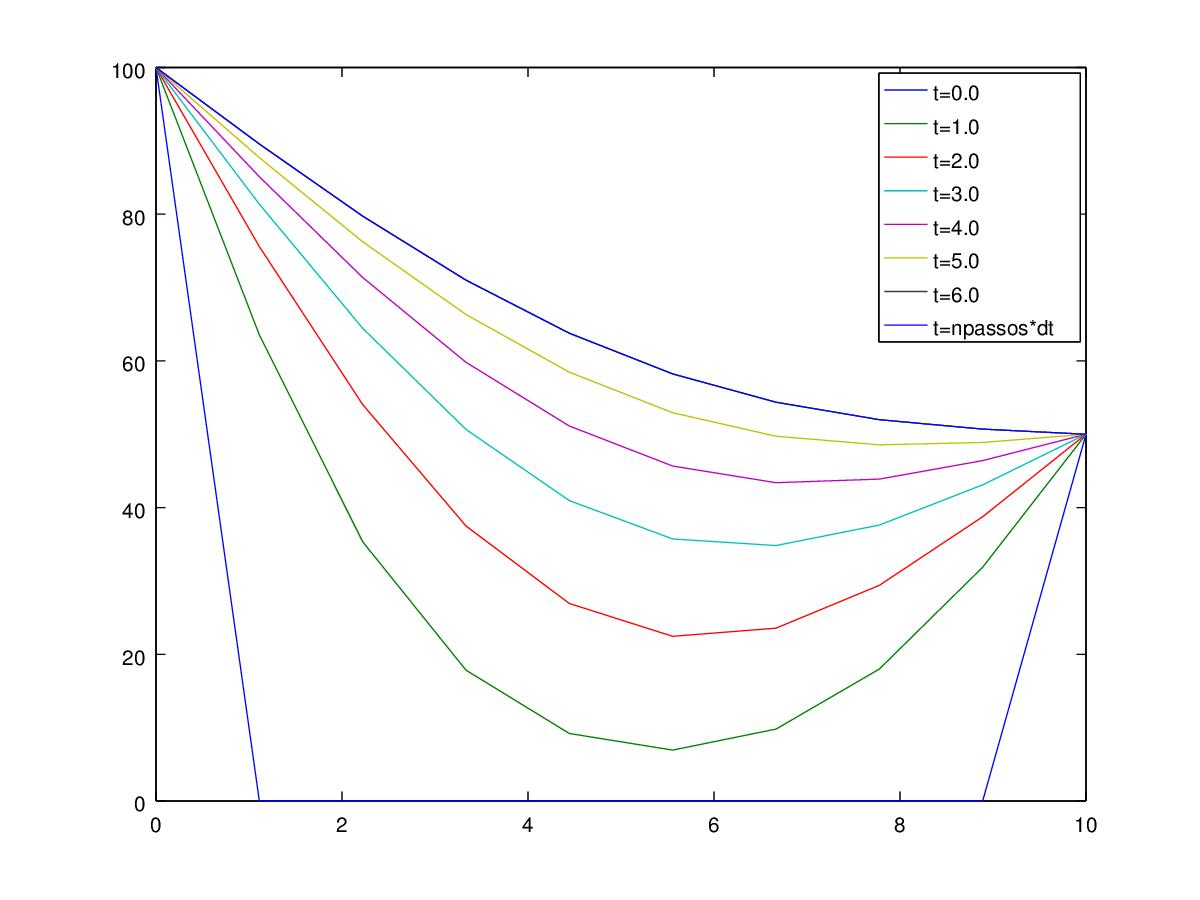
\includegraphics[width=0.8\textwidth]{teste1-imp-dt-04}
    \caption{Teste 1 - Alg. Implícito e $\Delta t = 0.4$}
    \label{fig:t1-imp}
\end{figure}

Na figura \ref{fig:t1-exp}, vemos o gráfico da solução obtida pelo 
algoritmo explícito, com $\Delta t = 0.8$. Vemos que o algoritmo implícito e 
este possuem gráficos muito díspares. O algoritmo Explícito, neste caso, 
apresentou este resultado devido à divergência. Com os parâmetros utilizados, 
não foi possível convergir, uma vez que o mesmo possui condições de 
estabilidade. Porém, reduzindo o delta, podemos alcançar a convergência.

\begin{figure}[ht]
    \centering
    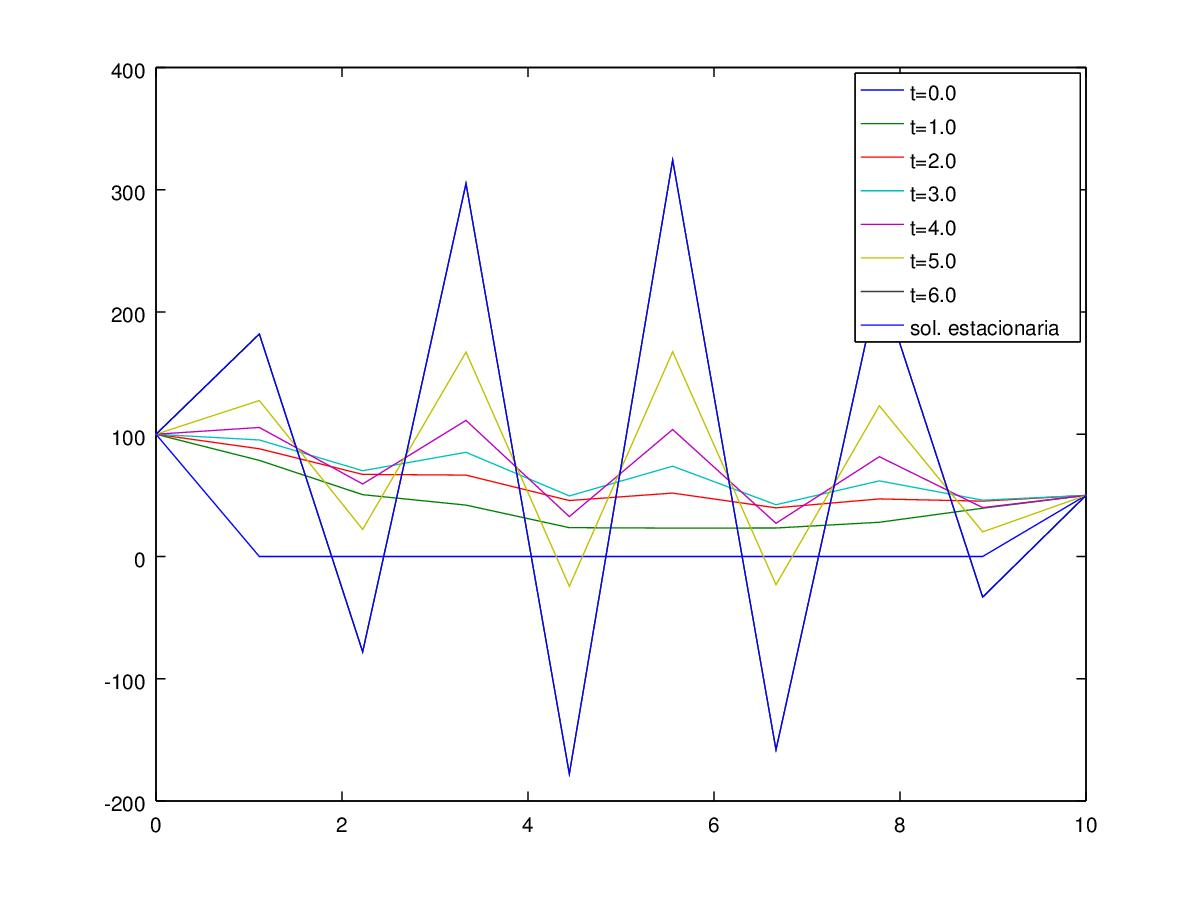
\includegraphics[width=0.8\textwidth]{teste1-exp-dt-08}
    \caption{Teste 1 - Alg. Explícito e $\Delta t = 0.8$}
    \label{fig:t1-exp}
\end{figure}

E na figura \ref{fig:t1-crank}, vemos o gráfico da solução obtida pelo 
algoritmo de Crank-Nicolson, com $\Delta t = 0.8$. Ao contrário do algoritmo 
explícito, o de Crank-Nicolson convergiu com os mesmo parâmetros. Além disto, 
vemos que obtemos uma convergência mais aparente. Podemos inferir que a solução 
é uma reta.

\begin{figure}[ht]
    \centering
    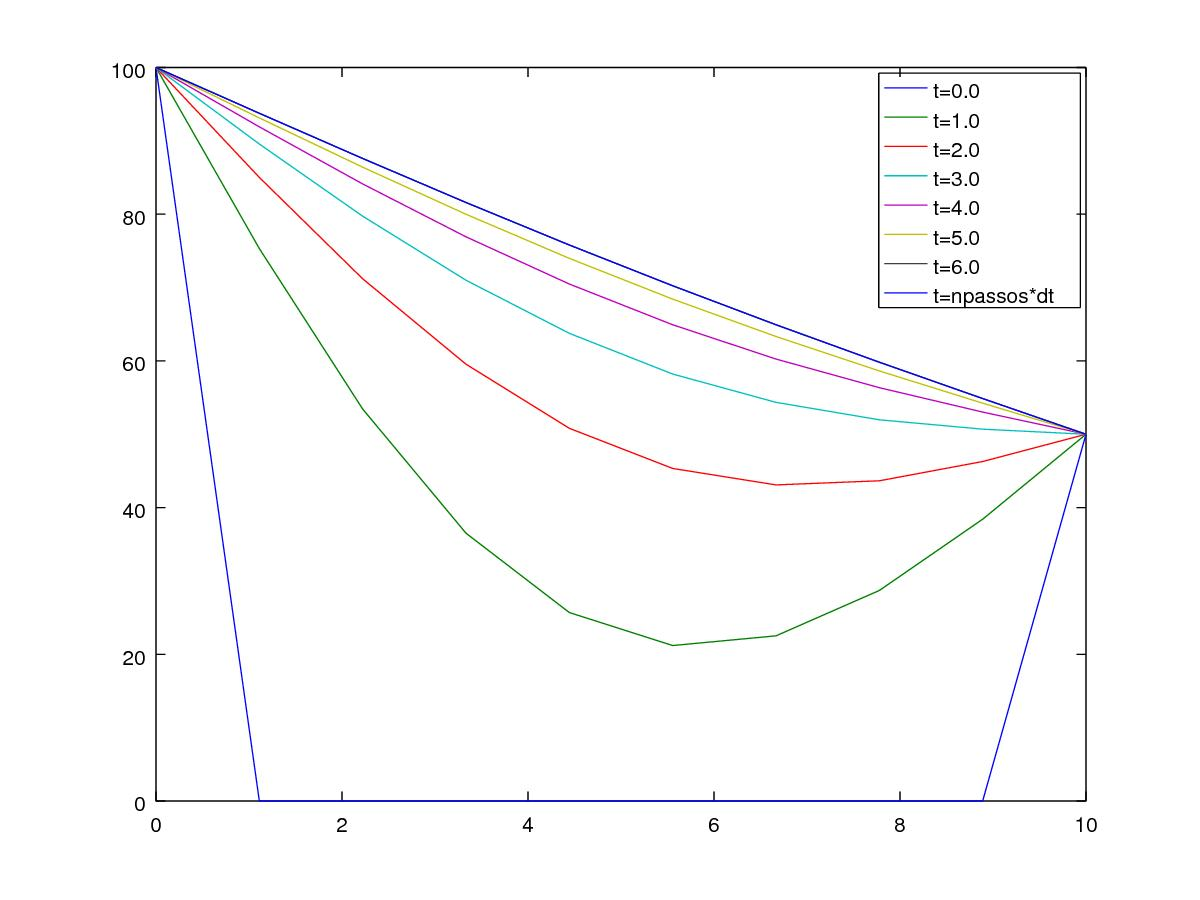
\includegraphics[width=0.8\textwidth]{teste1-crank-dt-08}
    \caption{Teste 1 - Alg. Crank-Nicolson e $\Delta t = 0.8$}
    \label{fig:t1-crank}
\end{figure}

\subsection{Teste 2}
Equação do calor com condutividade térmica $a(x,t) = 0.835 cm^2/s$ e fonte de 
calor nula:

\begin{itemize}
 \item Parâmetros básicos:
 $a(x,t) = 0.835$, $f(x,t) = 0$, $(0,l) = (0,10)$ e número de passos no tempo 
igual a 60.
 \item Condições de contorno e iniciais:
 $u(0,t) = 100ºC$, $\frac{\partial u(10,t)}{\partial x} = 0$ e 
$u(x,0) = 0$, para $x \in (0,10]$
 \item Parâmetros dos métodos de aproximação:
 \begin{itemize}
  \item $h = 1$ e $\Delta t_1 < \frac{h^2}{2a}$, $\Delta t_2 = 
\frac{h^2}{2a}$, $\Delta t_3 > \frac{h^2}{2a}$
  \item $h = 0.1$ e $\Delta t_1 < \frac{h^2}{2a}$, $\Delta t_2 = 
\frac{h^2}{2a}$, $\Delta t_3 > \frac{h^2}{2a}$
 \end{itemize}
\end{itemize}

Este teste é bastante similar ao primeiro, com a diferença que o extremo final 
do domínio não possui uma condição de contorno de valor prescrito, e sim com 
uma derivada conhecida.

Na figura \ref{fig:t2-imp}, vemos o gráfico da solução obtida pelo 
algoritmo implícito, com $\Delta t = 0.4$.

\begin{figure}[ht]
    \centering
    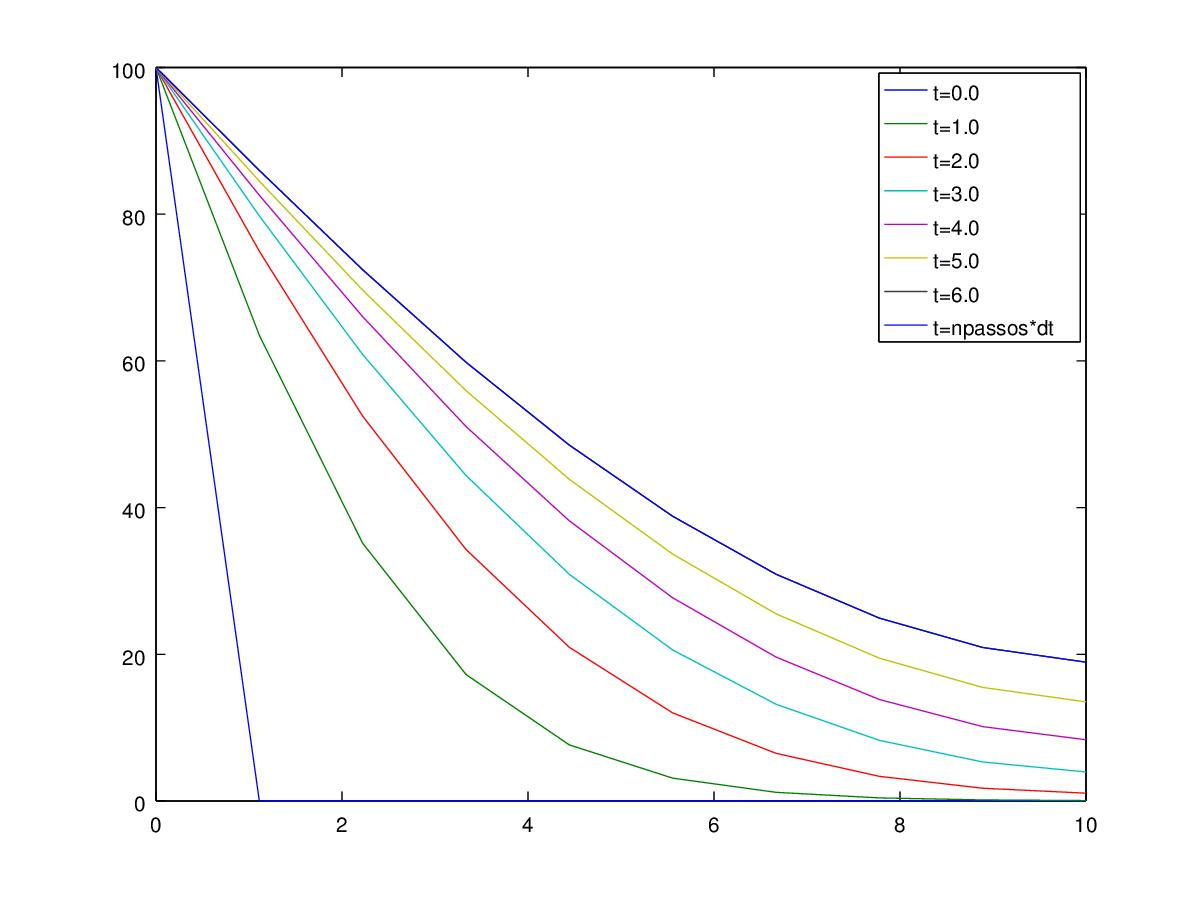
\includegraphics[width=0.8\textwidth]{teste2-imp-dt-04}
    \caption{Teste 2 - Alg. Implícito e $\Delta t = 0.4$}
    \label{fig:t2-imp}
\end{figure}

Na figura \ref{fig:t2-exp}, vemos o gráfico da solução obtida pelo 
algoritmo explícito, com $\Delta t = 0.5$. Este é muito similar ao do algoritmo 
implícito, e desta vez vemos que ele está \textit{convergindo}, assim como o 
implícito.

\begin{figure}[ht]
    \centering
    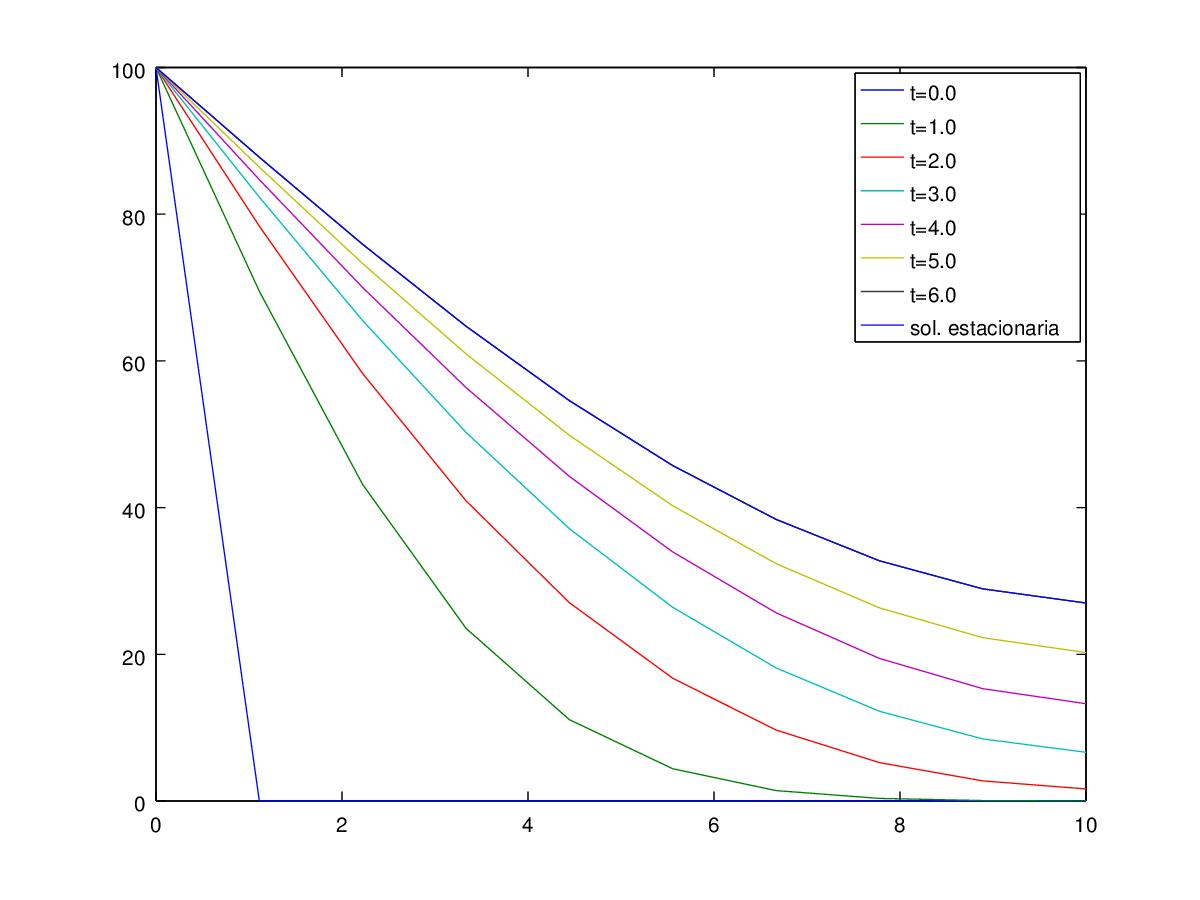
\includegraphics[width=0.8\textwidth]{teste2-exp-dt-05}
    \caption{Teste 2 - Alg. Explícito e $\Delta t = 0.5$}
    \label{fig:t2-exp}
\end{figure}

Até este momento, com estas soluções obtidas, não conseguimos dizer qual é a 
solução exata, uma vez que é possível observar que as curvas apresentadas não 
demonstram convergência. Isto se deve ao fato de que o número de passo $60$ é 
muito pequeno para este caso.

Portanto, na figura \ref{fig:t2-crank}, vemos o gráfico da solução obtida pelo 
algoritmo de Crank-Nicolson, com $\Delta t = 0.4$ e o número de passo igual a 
600. Desta forma, é notável que a solução tende à constante $100$. Isto era 
esperado pois temos a derivada conhecida $\frac{\partial u(10,t)}{\partial x} = 
0$ e $u(0,t) = 100$. Ou seja, a função deve começar em $100$ e terminar com 
derivada em $x$ nula, que é um reta horizontal.

\begin{figure}[ht]
    \centering
    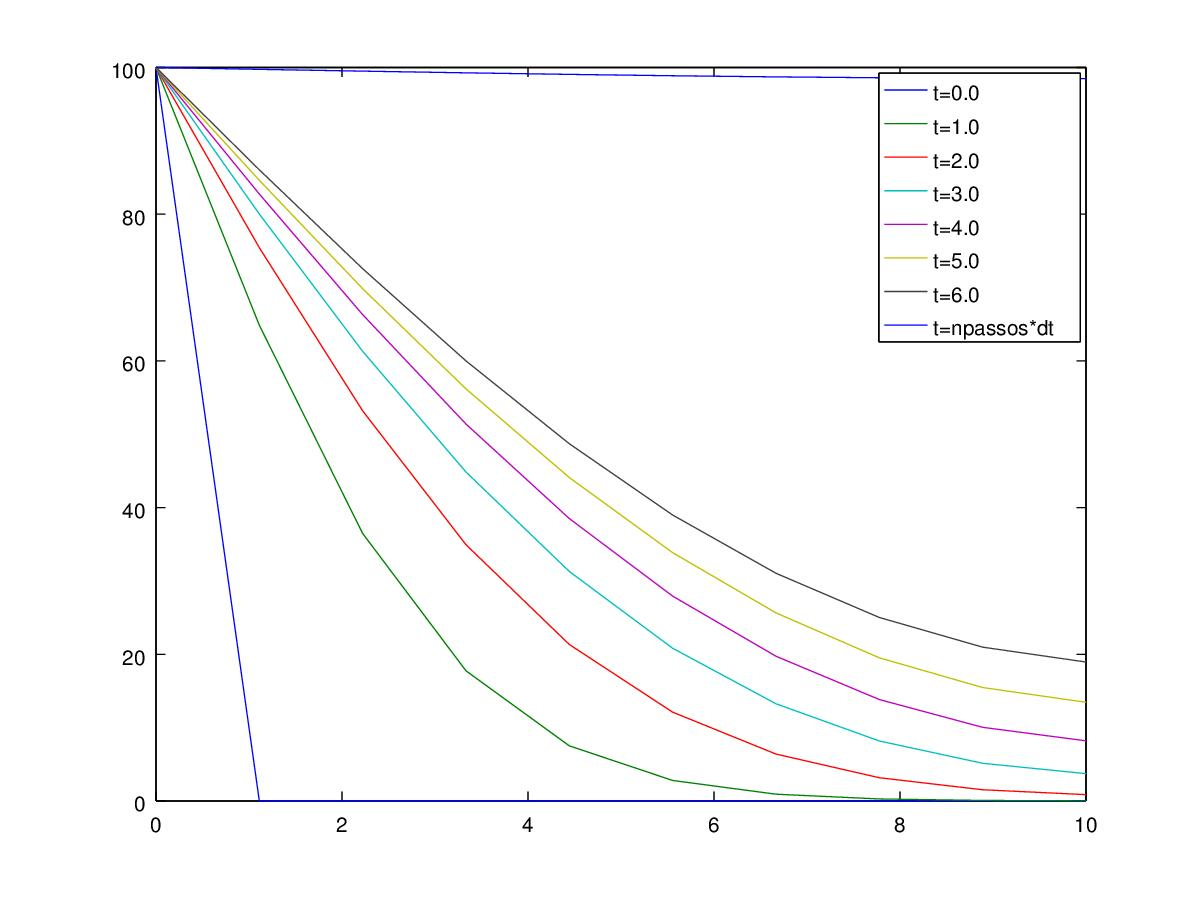
\includegraphics[width=0.8\textwidth]{teste2-crank-dt-04}
    \caption{Teste 2 - Alg. Crank-Nicolson e $\Delta t = 0.4$}
    \label{fig:t2-crank}
\end{figure}

\subsection{Teste 3}
Equação do calor com condutividade térmica $a(x,t) = 0.835 cm^2/s$ e fonte de 
calor unitária:

\begin{itemize}
 \item Parâmetros básicos:
 $a(x,t) = 0.835$, $f(x,t) = 1$, $(0,l) = (0,10)$ e número de passos no tempo 
igual a 60.
 \item Condições de contorno e iniciais:
 $u(0,t) = 100ºC$, $\frac{\partial u(10,t)}{\partial x} = 0$ e 
$u(x,0) = 0$, para $x \in (0,10]$
 \item Parâmetros dos métodos de aproximação:
 \begin{itemize}
  \item $h = 1$ e $\Delta t_1 < \frac{h^2}{2a}$, $\Delta t_2 = 
\frac{h^2}{2a}$, $\Delta t_3 > \frac{h^2}{2a}$
  \item $h = 0.1$ e $\Delta t_1 < \frac{h^2}{2a}$, $\Delta t_2 = 
\frac{h^2}{2a}$, $\Delta t_3 > \frac{h^2}{2a}$
 \end{itemize}
\end{itemize}

Este teste é similar ao segundo, com a diferença que agora temos fonte de 
calor igual à $1$, que antes era nula.

Na figura \ref{fig:t3-imp}, vemos o gráfico da solução obtida pelo 
algoritmo implícito, com $\Delta t = 0.8$.

\begin{figure}[ht]
    \centering
    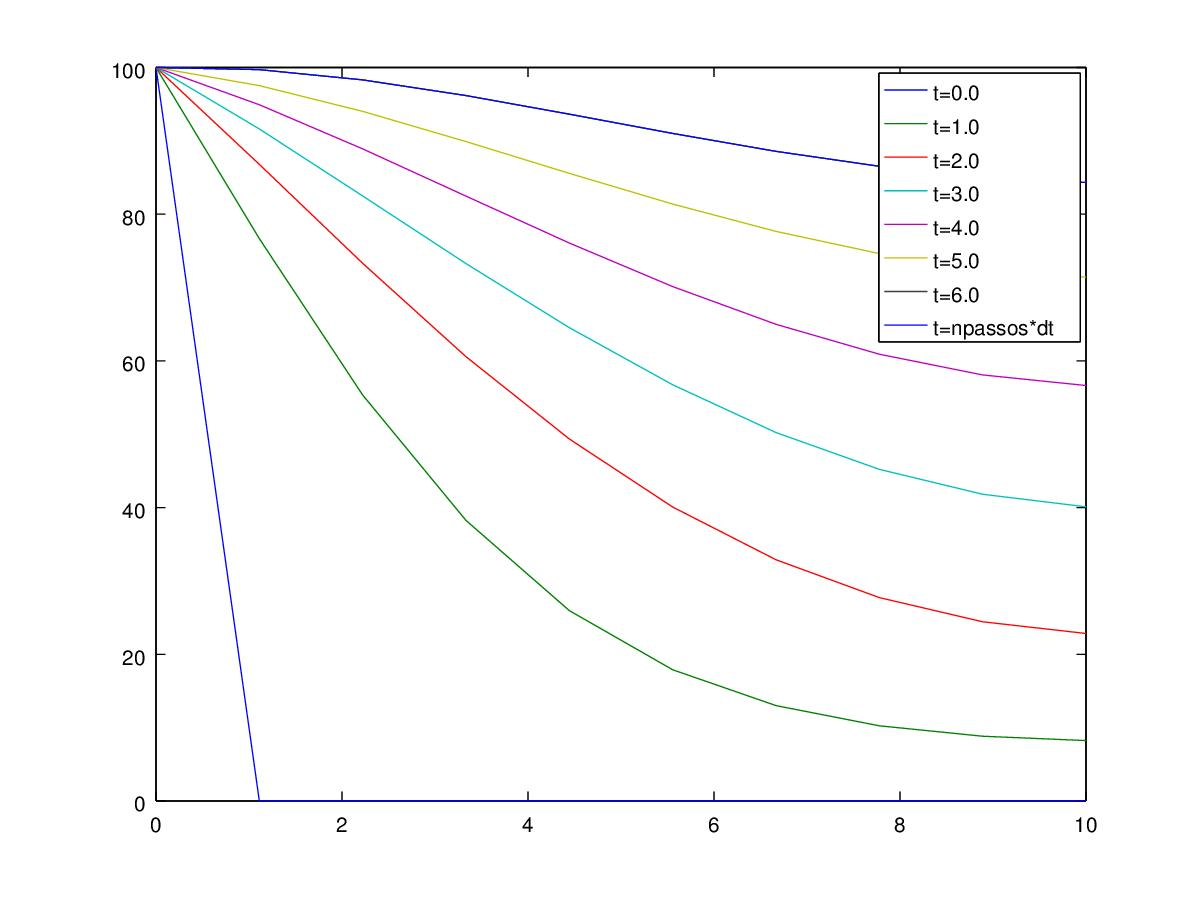
\includegraphics[width=0.8\textwidth]{teste3-imp-dt-08}
    \caption{Teste 2 - Alg. Implícito e $\Delta t = 0.8$}
    \label{fig:t3-imp}
\end{figure}

Na figura \ref{fig:t3-exp}, vemos o gráfico da solução obtida pelo 
algoritmo explícito, com $\Delta t = 0.5$.

\begin{figure}[ht]
    \centering
    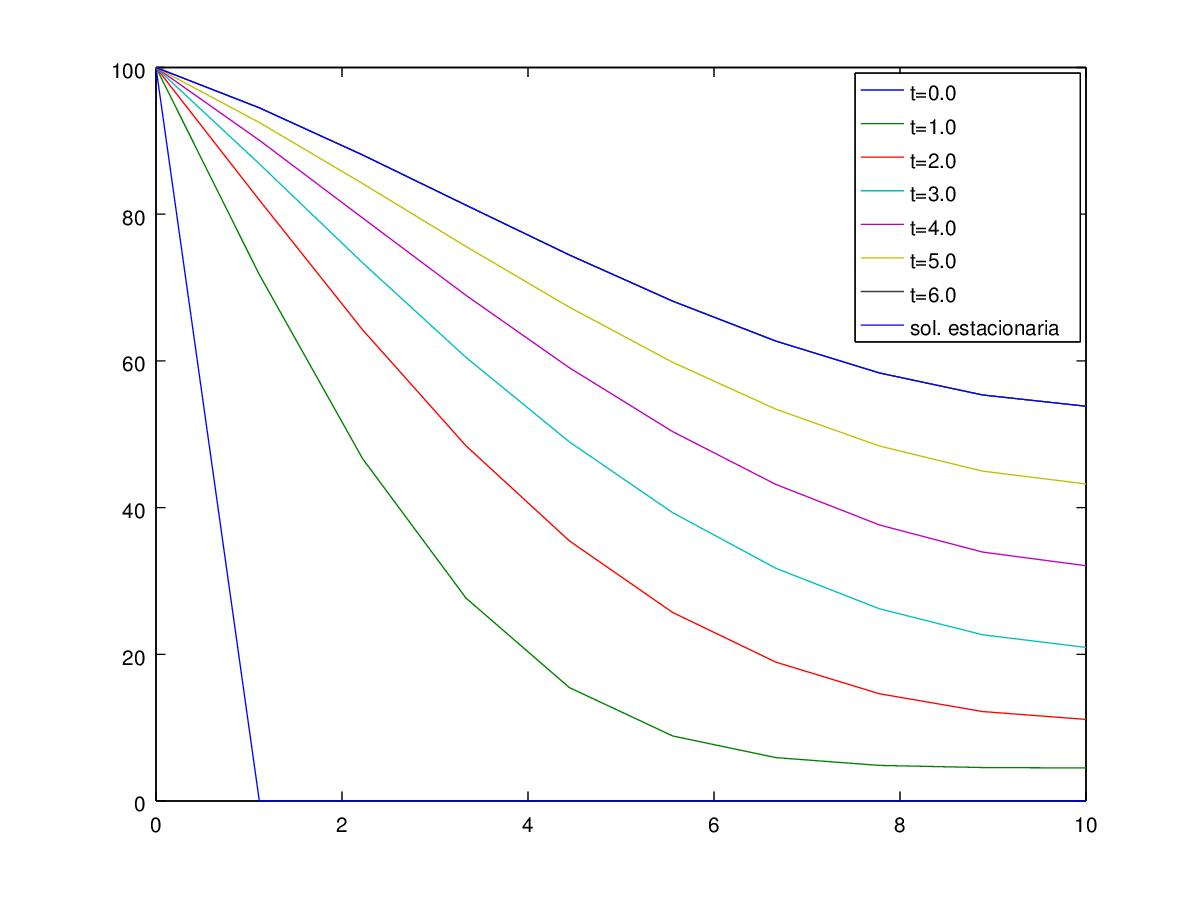
\includegraphics[width=0.8\textwidth]{teste3-exp-dt-05}
    \caption{Teste 2 - Alg. Explícito e $\Delta t = 0.5$}
    \label{fig:t3-exp}
\end{figure}

Mais uma vez não conseguimos dizer qual é a solução exata. devido ao fato de 
que o número de passo $60$ é muito pequeno.

Portanto, na figura \ref{fig:t3-crank}, vemos o gráfico da solução obtida pelo 
algoritmo de Crank-Nicolson, com $\Delta t = 0.4$ e o número de passo igual a 
$600$. Com isto, podemos observar que o comportamento da solução é bem 
diferente do aparente até então. O que acontece de fato é que a curva tende à 
uma parábola.

\begin{figure}[ht]
    \centering
    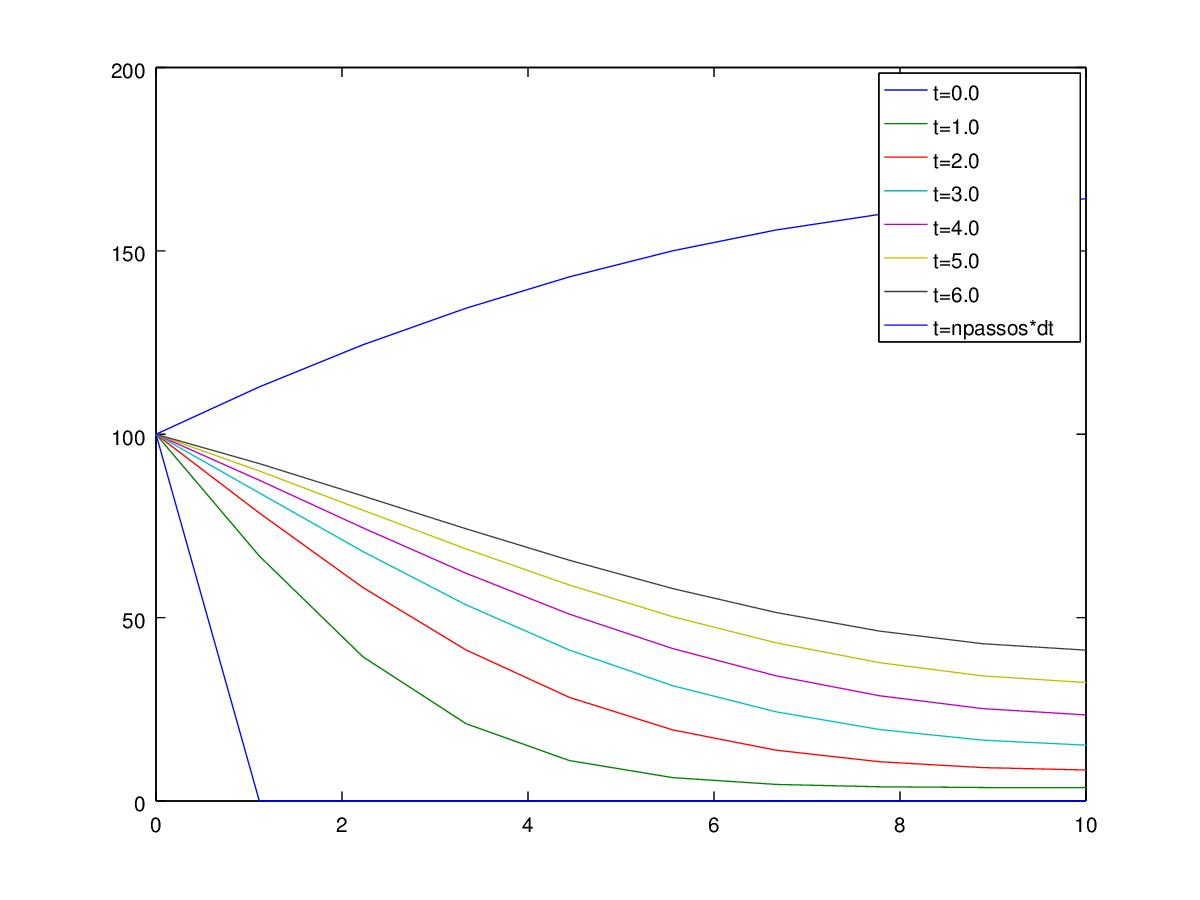
\includegraphics[width=0.8\textwidth]{teste3-crank-dt-04}
    \caption{Teste 2 - Alg. Crank-Nicolson e $\Delta t = 0.4$}
    \label{fig:t3-crank}
\end{figure}

% ------------------------------------------------------------------------------
% Conclusão
% ------------------------------------------------------------------------------
\section{Conclusão}
Os algoritmos apresentados são todos passíveis de uso, devendo apenas 
considerar algumas questões específicas. O algoritmo Explícito possui o 
limitador de caracterizar-se como um procedimento condicionalmente estável. Ou 
seja, existem restrições a serem atendidas para que o processo seja 
convergente. Logo, não é sempre viável escolher este método para a solução.

Tanto o método Implícito quando o de Crank-Nicolson são incondicionalmente 
estáveis. Isto que dizer que não apresentam restrições como o Explícito. 
Portanto seu uso é mais plausível quando não temos um problema específico 
conhecido.

Em relação ao valor de $\Delta t$, nota-se que existe um intervalo indicado 
para a sua escolha. Caso seja atribuindo um valor grande, teremos soluções 
incoerentes. E caso seja um valor muito pequeno, a convergência será muito 
lenta. Os valores ``ideais'' estariam entre 0.5 e 1, onde apresentam uma boa 
taxa de convergência.

\end{document}
